\let\negmedspace\undefined
\let\negthickspace\undefined
\documentclass[journal]{IEEEtran}
\usepackage[a5paper, margin=10mm, onecolumn]{geometry}
%\usepackage{lmodern} % Ensure lmodern is loaded for pdflatex
\usepackage{tfrupee} % Include tfrupee package

\setlength{\headheight}{1cm} % Set the height of the header box
\setlength{\headsep}{0mm}     % Set the distance between the header box and the top of the text

\usepackage{gvv-book}
\usepackage{gvv}
\usepackage{cite}
\usepackage{amsmath,amssymb,amsfonts,amsthm}
\usepackage{algorithmic}
\usepackage{graphicx}
\usepackage{textcomp}
\usepackage{xcolor}
\usepackage{txfonts}
\usepackage{listings}
\usepackage{enumitem}
\usepackage{mathtools}
\usepackage{gensymb}
\usepackage{comment}
%\usepackage{multiclo}
\usepackage[breaklinks=true]{hyperref}
\usepackage{tkz-euclide} 
\usepackage{listings}
% \usepackage{gvv} 
\graphicspath{ {./figs/} }

\begin{document}

\title{
ME: MECHANICAL ENGINEERING}
\author{AI25BTECH11011}
\maketitle
\renewcommand{\thefigure}{\theenumi}
\renewcommand{\thetable}{\theenumi}

\textbf{Q.1 - Q.25 carry one mark each.}

\begin{enumerate}

\item A streamline and an equipotential line in a flow field
\begin{enumerate}
\item are parallel to each other  
\item are perpendicular to each other  
\item intersect at an acute angle  
\item are identical  
\end{enumerate}
\hfill (GATE ME 2011)

\item If a mass of moist air in an airtight vessel is heated to a higher temperature, then
\begin{enumerate}
\item specific humidity of the air increases  
\item specific humidity of the air decreases  
\item relative humidity of the air increases  
\item relative humidity of the air decreases  
\end{enumerate}
\hfill (GATE ME 2011)

\item In a condenser of a power plant, the steam condenses at a temperature of $60^\circ\text{C}$. The cooling water enters at $30^\circ\text{C}$ and leaves at $45^\circ\text{C}$. The logarithmic mean temperature difference (LMTD) of the condenser is
\begin{multicols}{4}
\begin{enumerate}
\item $16.2^\circ\text{C}$  
\item $21.6^\circ\text{C}$  
\item $30^\circ\text{C}$  
\item $37.5^\circ\text{C}$  
\end{enumerate}
\end{multicols} 
\hfill (GATE ME 2011)              

\item A simply supported beam PQ is loaded by a moment of 1 kN-m at the mid-span of the beam as shown in the figure. The reaction forces $R_P$ and $R_Q$ at supports P and Q respectively are

\begin{figure}[H]
    \centering
    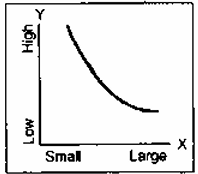
\includegraphics[width=0.8\textwidth]{Fig 1.png}
    \caption{}
    \label{fig:question4}
\end{figure}

\begin{multicols}{2}
\begin{enumerate}
\item 1 kN downward, 1 kN upward  
\item 0.5 kN upward, 0.5 kN downward  
\item 0.5 kN downward, 0.5 kN upward  
\item 1 kN upward, 1 kN upward  
\end{enumerate}
\end{multicols} 
\hfill (GATE ME 2011)              

\item A double-parallelogram mechanism is shown in the figure. Note that PQ is a single link. The mobility of the mechanism is

\begin{figure}[H]
    \centering
    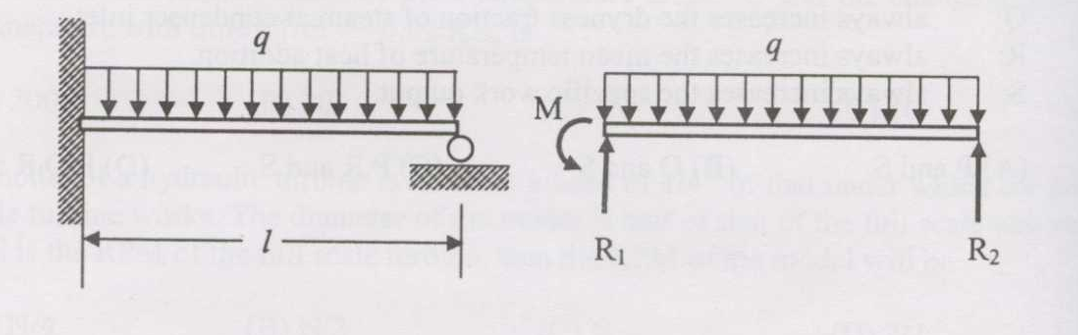
\includegraphics[width=0.8\textwidth]{Fig 2.png}
    \caption{}
    \label{fig:question5}
\end{figure}

\begin{multicols}{4}
\begin{enumerate}
\item $-1$  
\item 0  
\item 1  
\item 2  
\end{enumerate}
\end{multicols}   
\hfill (GATE ME 2011)                 

\item The maximum possible draft in cold rolling of sheet increases with the
\begin{enumerate}
\item increase in coefficient of friction  
\item decrease in coefficient of friction  
\item decrease in roll radius  
\item increase in roll velocity  
\end{enumerate}   
\hfill (GATE ME 2011)

\item The operation in which oil is permeated into the pores of a powder metallurgy product is known as
\begin{multicols}{4}
\begin{enumerate}
\item mixing  
\item sintering  
\item impregnation  
\item infiltration  
\end{enumerate}
\end{multicols}   
\hfill (GATE ME 2011)                 

\item A hole is of dimension $9^{+0.015}_{+0}$ mm. The corresponding shaft is of dimension $\phi9^{+0.010}_{+0.001}$ mm. The resulting assembly has
\begin{multicols}{2}
\begin{enumerate}
\item loose running fit  
\item close running fit  
\item transition fit  
\item interference fit  
\end{enumerate}
\end{multicols}   
\hfill (GATE ME 2011)               

\item Heat and work are
\begin{multicols}{2}
\begin{enumerate}
\item intensive properties  
\item extensive properties  
\item point functions  
\item path functions  
\end{enumerate}
\end{multicols}   
\hfill (GATE ME 2011)               

\item A column has a rectangular cross-section of $10\,\text{mm} \times 20\,\text{mm}$ and a length of $1\,\text{m}$. The slenderness ratio of the column is close to
\begin{multicols}{4}
\begin{enumerate}
\item 200  
\item 346  
\item 477  
\item 1000  
\end{enumerate}
\end{multicols}   
\hfill (GATE ME 2011)               

\item A series expansion for the function $\sin \theta$ is
\begin{multicols}{2}
\begin{enumerate}
\item $ 1 - \frac{\theta^2}{2!} + \frac{\theta^4}{4!} - \cdots $
\item $ \theta - \frac{\theta^3}{3!} + \frac{\theta^5}{5!} - \cdots $
\item $ 1 + \theta + \frac{\theta^2}{2!} + \frac{\theta^3}{3!} + \cdots $
\item $ \theta + \frac{\theta^3}{3!} + \frac{\theta^5}{5!} + \cdots $
\end{enumerate}
\end{multicols}    
\hfill (GATE ME 2011)  

\item Green sand mould indicates that
\begin{multicols}{2}
\begin{enumerate}
\item polymeric mould has been cured  
\item mould has been totally dried  
\item mould is green in colour  
\item mould contains moisture  
\end{enumerate}
\end{multicols}    
\hfill (GATE ME 2011)  

\item What is $\lim_{\theta \to 0} \frac{\sin \theta}{\theta}$ equal to?
\begin{multicols}{4}
\begin{enumerate}
\item $\theta$  
\item $\sin \theta$  
\item $0$  
\item $1$  
\end{enumerate}
\end{multicols}    
\hfill (GATE ME 2011)  

\item Eigenvalues of a real symmetric matrix are always
\begin{multicols}{4}
\begin{enumerate}
\item positive  
\item negative  
\item real  
\item complex  
\end{enumerate}
\end{multicols}    
\hfill (GATE ME 2011)  

\item A pipe of 25 mm outer diameter carries steam. The heat transfer coefficient between the cylinder and surroundings is $5\,\text{W/m}^2\text{K}$. It is proposed to reduce the heat loss from the pipe by adding insulation having a thermal conductivity of $0.05\,\text{W/mK}$. Which one of the following statements is \textbf{TRUE}?
\begin{enumerate}
\item The outer radius of the pipe is equal to the critical radius.  
\item The outer radius of the pipe is less than the critical radius.  
\item Adding the insulation will reduce the heat loss.  
\item Adding the insulation will increase the heat loss.  
\end{enumerate}
\hfill (GATE ME 2011)

\item The contents of a well-insulated tank are heated by a resistor of $23\,\Omega$ in which $10\,\text{A}$ current is flowing. Consider the tank along with its contents as a thermodynamic system. The work done by the system and the heat transfer to the system are positive. The rates of heat ($Q$), work ($W$) and change in internal energy ($\Delta U$) during the process in kW are
\begin{multicols}{2}
\begin{enumerate}
\item $Q = 0$, $W = -2.3$, $\Delta U = +2.3$  
\item $Q = +2.3$, $W = 0$, $\Delta U = +2.3$  
\item $Q = -2.3$, $W = 0$, $\Delta U = -2.3$  
\item $Q = 0$, $W = +2.3$, $\Delta U = -2.3$  
\end{enumerate}
\end{multicols}   
\hfill (GATE ME 2011)  

\item Match the following criteria of material failure, under biaxial stresses $\sigma_1$ and $\sigma_2$ and yield stress $\sigma_y$, with their corresponding graphic representations:

\begin{figure}[H]
    \centering
    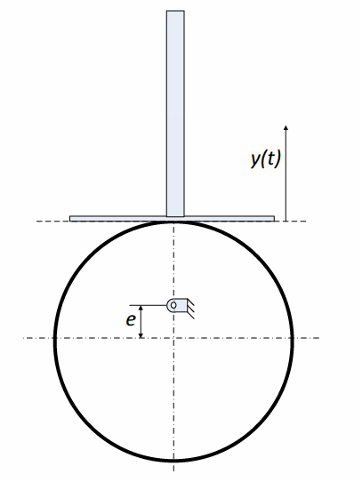
\includegraphics[width=0.8\textwidth]{Fig 3.png}
    \caption{}
    \label{fig:question17}
\end{figure}

\begin{multicols}{2}
\begin{enumerate}
\item P-M, Q-L, R-N  
\item P-N, Q-M, R-L  
\item P-M, Q-N, R-L  
\item P-N, Q-L, R-M  
\end{enumerate}
\end{multicols}   
\hfill (GATE ME 2011)  

\item The product of two complex numbers $1+i$ and $2-5i$ is
\begin{multicols}{2}
\begin{enumerate}
\item $7 - 3i$  
\item $3 - 4i$  
\item $-3 - 4i$  
\item $7 + 3i$  
\end{enumerate}
\end{multicols}   
\hfill (GATE ME 2011)  

\item Cars arrive at a service station according to Poisson's distribution with a mean rate of 5 per hour. The service time per car is exponential with a mean of 10 minutes. At steady state, the average waiting time in the queue is
\begin{multicols}{4}
\begin{enumerate}
\item 10 minutes  
\item 20 minutes  
\item 25 minutes  
\item 50 minutes  
\end{enumerate} 
\end{multicols}   
\hfill (GATE ME 2011)  

\item The word \textbf{kanban} is most appropriately associated with
\begin{multicols}{2}
\begin{enumerate}
\item economic order quantity  
\item just-in-time production  
\item capacity planning  
\item product design  
\end{enumerate}
\end{multicols}   
\hfill (GATE ME 2011)  

\item If $f(x)$ is an even function and $a$ is a positive real number, then $\int_{-a}^{a} f(x)\,dx$ equals
\begin{multicols}{4}
\begin{enumerate}
\item 0  
\item $a$  
\item $2a$  
\item 2 $\int_{a}^{0} f(x)\,dx$   
\end{enumerate}
\end{multicols}   
\hfill (GATE ME 2011)  

\item The coefficient of restitution of a perfectly plastic impact is
\begin{multicols}{4}
\begin{enumerate}
\item 0  
\item 1  
\item 2  
\item $\infty$
\end{enumerate}
\end{multicols}   
\hfill (GATE ME 2011)  

\item A thin cylinder of inner radius 500 mm and thickness 10 mm is subjected to an internal pressure of 5 MPa. The average circumferential (hoop) stress in MPa is
\begin{multicols}{4}
\begin{enumerate}
\item 100  
\item 250  
\item 500  
\item 1000  
\end{enumerate}
\end{multicols}  
\hfill (GATE ME 2011)  

\item Which one among the following welding processes uses non-consumable electrode?
\begin{multicols}{2}
\begin{enumerate}
\item Gas metal arc welding  
\item Submerged arc welding  
\item Gas tungsten arc welding  
\item Flux coated arc welding  
\end{enumerate}
\end{multicols}  
\hfill (GATE ME 2011)  

\item The crystal structure of austenite is
\begin{multicols}{2}
\begin{enumerate}
\item body centered cubic  
\item face centered cubic  
\item hexagonal closed packed  
\item body centered tetragonal  
\end{enumerate}
\end{multicols}  
\hfill (GATE ME 2011)  

\textbf{Q.26 to Q.55 carry two marks each.}

\item A torque $ T $ is applied at the free end of a stepped rod of circular cross-sections as shown in the figure. The shear modulus of the material of the rod is $ G $. The expression for $ d $ to produce an angular twist $ \theta $ at the free end is:

\begin{figure}[H]
    \centering
    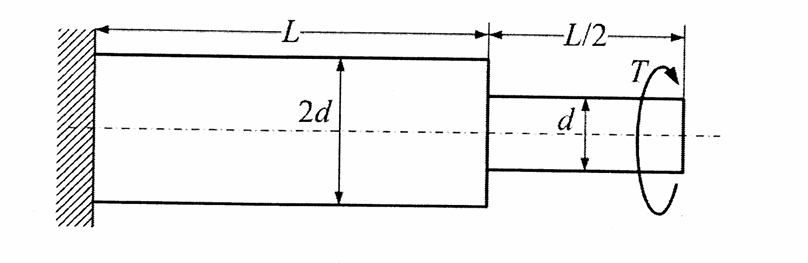
\includegraphics[width=0.8\textwidth]{Fig 4.png}
    \caption{}
    \label{fig:question26}
\end{figure}

\begin{multicols}{4}
\begin{enumerate}
\item $ \left( \frac{32TL}{\pi \theta G} \right)^{\frac{1}{4}} $
\item $ \left( \frac{18TL}{\pi \theta G} \right)^{\frac{1}{4}} $
\item $ \left( \frac{16TL}{\pi \theta G} \right)^{\frac{1}{4}} $
\item $ \left( \frac{2TL}{\pi \theta G} \right)^{\frac{1}{4}} $
\end{enumerate}
\end{multicols}  
\hfill (GATE ME 2011)

\item Figure shows the schematic for the measurement of velocity of air (density = $1.2\,\text{kg/m}^3$) through a constant-area duct using a pitot tube and a water-tube manometer. The differential head of water (density = $1000\,\text{kg/m}^3$) in the two columns of the manometer is 10 mm. Take acceleration due to gravity as $9.8\,\text{m/s}^2$. The velocity of air in m/s is:

\begin{figure}[H]
    \centering
    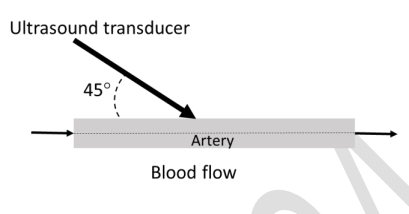
\includegraphics[width=0.8\textwidth]{Fig 5.png}
    \caption{}
    \label{fig:question27}
\end{figure}

\begin{multicols}{4}
\begin{enumerate}
\item 6.4  
\item 9.0  
\item 12.8  
\item 25.6  
\end{enumerate}
\end{multicols}  
\hfill (GATE ME 2011)

\item The values of enthalpy of steam at the inlet and outlet of a steam turbine in a Rankine cycle are 2800 kJ/kg and 1800 kJ/kg respectively. Neglecting pump work, the specific steam consumption in kg/kW-hour is:

\begin{multicols}{4}
\begin{enumerate}
\item 3.60  
\item 0.36  
\item 0.06  
\item 0.01  
\end{enumerate}
\end{multicols}  
\hfill (GATE ME 2011)

\item The integral $\int_1^3 \frac{1}{x}\,dx$, when evaluated by using Simpson's 1/3 rule on two equal subintervals each of length 1, equals
\begin{multicols}{4}
\begin{enumerate}
\item 1.000  
\item 1.098  
\item 1.111  
\item 1.120  
\end{enumerate}
\end{multicols}  
\hfill (GATE ME 2011)  

\item Two identical ball bearings P and Q are operating at loads 30 kN and 45 kN respectively. The ratio of the life of bearing P to the life of bearing Q is
\begin{multicols}{4}
\begin{enumerate}
\item $81/16$  
\item $27/8$  
\item $9/4$  
\item $3/2$  
\end{enumerate}
\end{multicols}  
\hfill (GATE ME 2011)  

\item For the four-bar linkage shown in the figure, the angular velocity of link AB is 1 rad/s. The length of link CD is 1.5 times the length of link AB. In the configuration shown, the angular velocity of link CD in rad/s is:

\begin{figure}[H]
    \centering
    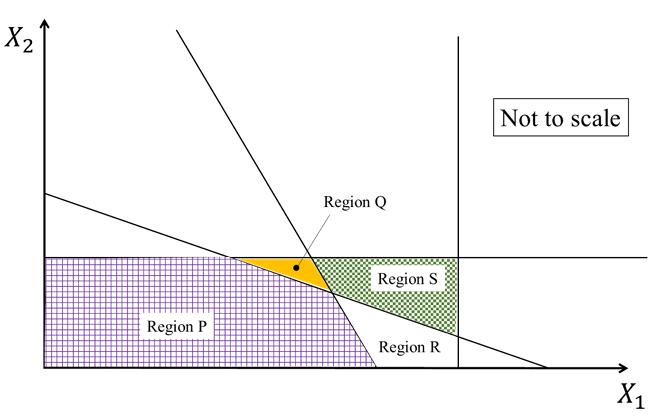
\includegraphics[width=0.8\textwidth]{Fig 6.png}
    \caption{}
    \label{fig:question31}
\end{figure}

\begin{multicols}{4}
\begin{enumerate}
\item 3  
\item $ \frac{3}{2} $  
\item 1  
\item $ \frac{2}{3} $  
\end{enumerate}
\end{multicols}  
\hfill (GATE ME 2011)

\item A stone with mass of 0.1 kg is catapulted as shown in the figure. The total force $ F_x $ (in N) exerted by the rubber band as a function of distance $ x $ (in m) is given by $ F_x = 300x^2 $. If the stone is displaced by 0.1 m from the un-stretched position, the energy stored in the rubber band is:

\begin{figure}[H]
    \centering
    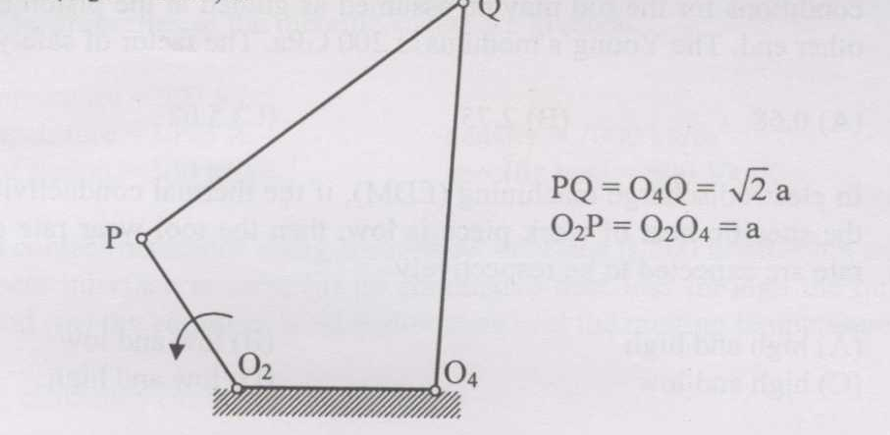
\includegraphics[width=0.8\textwidth]{Fig 7.png}
    \caption{}
    \label{fig:question32}
\end{figure}

\begin{multicols}{4}
\begin{enumerate}
\item 0.01 J  
\item 0.1 J  
\item 1 J  
\item 10 J  
\end{enumerate}
\end{multicols}   
\hfill (GATE ME 2011)

\item Consider the differential equation $ \frac{dy}{dx} = (1 + y^2)x $. The general solution with constant $ c $ is:
\begin{multicols}{2}
\begin{enumerate}
\item $ y = \tan \frac{x^2}{2} + \tan c $
\item $ y = \tan^2\left( \frac{x}{2} + c \right) $  
\item $ y = \tan^2( \frac{x}{2}) + c  $  
\item $ y = \tan\left(\frac{x^2}{2} + c \right) $  
\end{enumerate}
\end{multicols}   
\hfill (GATE ME 2011)

\item An unbiased coin is tossed five times. The outcome of each toss is either a head or a tail. The probability of getting at least one head is:
\begin{multicols}{4}
\begin{enumerate}
\item $ \frac{1}{32} $  
\item $ \frac{13}{32} $  
\item $ \frac{16}{32} $  
\item $ \frac{31}{32} $  
\end{enumerate}
\end{multicols}   
\hfill (GATE ME 2011)

\item A mass of 1 kg is attached to two identical springs each with stiffness $ k = 20\,\text{kN/m} $ as shown in the figure. Under frictionless condition, the natural frequency of the system in Hz is close to:

\begin{figure}[H]
    \centering
    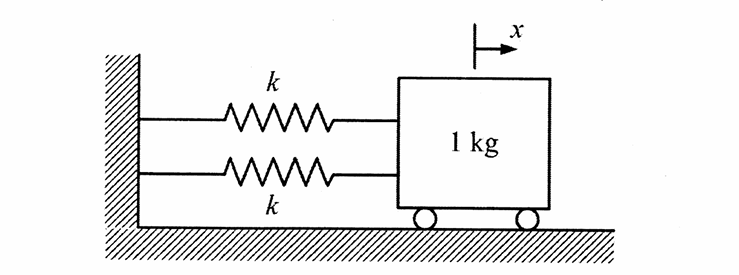
\includegraphics[width=0.8\textwidth]{Fig 8.png}
    \caption{}
    \label{fig:question35}
\end{figure}

\begin{multicols}{4}
\begin{enumerate}
\item 32  
\item 23  
\item 16  
\item 11  
\end{enumerate}
\end{multicols}   
\hfill (GATE ME 2011)

\item The shear strength of a sheet metal is 300 MPa. The blanking force required to produce a blank of 100 mm diameter from a 1.5 mm thick sheet is close to:
\begin{multicols}{4}
\begin{enumerate}
\item 45 kN  
\item 70 kN  
\item 141 kN  
\item 3500 kN  
\end{enumerate}
\end{multicols}   
\hfill (GATE ME 2011)

\item The ratios of the laminar hydrodynamic boundary layer thickness to thermal boundary layer thickness of flows of two fluids P and Q on a flat plate are $ \frac{1}{2} $ and 2 respectively. The Reynolds number for both flows is $ 10^4 $. The Prandtl and Nusselt numbers for P are $ \frac{1}{8} $ and 35 respectively. The Prandtl and Nusselt numbers for Q are respectively:
\begin{multicols}{4}
\begin{enumerate}
\item 8 and 140  
\item 8 and 70  
\item 4 and 70  
\item 4 and 35  
\end{enumerate}
\end{multicols}    
\hfill (GATE ME 2011)

\item The crank radius of a single-cylinder I.C. engine is 60 mm and the diameter of the cylinder is 80 mm. The swept volume of the cylinder in cm$^3$ is:
\begin{multicols}{4}
\begin{enumerate}
\item 48  
\item 96  
\item 302  
\item 603  
\end{enumerate}
\end{multicols}    
\hfill (GATE ME 2011)

\item A pump raises liquid pressure from 1 bar to 30 bar. Density of liquid is 990 kg/m$^3$. The isentropic specific work done by the pump in kJ/kg is:
\begin{multicols}{4}
\begin{enumerate}
\item 0.10  
\item 0.30  
\item 2.50  
\item 2.93  
\end{enumerate}
\end{multicols}    
\hfill (GATE ME 2011)

\item A spherical steel ball of 12 mm diameter is initially at 1000 K. It is slowly cooled in a surrounding of 300 K. Heat transfer coefficient is 5 W/m$^2$K, and thermal conductivity of steel is 20 W/mK. The temperature difference between the centre and surface of the ball is:
\begin{enumerate}
\item Large because conduction resistance is far higher than convective resistance  
\item Large because conduction resistance is far less than convective resistance  
\item Small because conduction resistance is far higher than convective resistance  
\item Small because conduction resistance is far less than convective resistance  
\end{enumerate}
\hfill (GATE ME 2011)

\item An ideal Brayton cycle operates between the pressure limits of  1 bar and 6 bar, has minimum and maximum temperatures 300 K and 1500 K. The ratio of specific heats of the working fluid is 1.4. The approximate final temperatures in Kelvin at the end of compression and expansion are respectively
\begin{multicols}{4}
\begin{enumerate}
\item 500 and 900  
\item 900 and 500  
\item 500 and 500  
\item 900 and 900  
\end{enumerate}
\end{multicols}   
\hfill (GATE ME 2011)

\item A disc of mass $ m $ is attached to a spring of stiffness $ k $  as shown in the figure. The disc rolls without slipping on a horizontal surface. The natural frequency of vibration of the system is:

\begin{figure}[H]
    \centering
    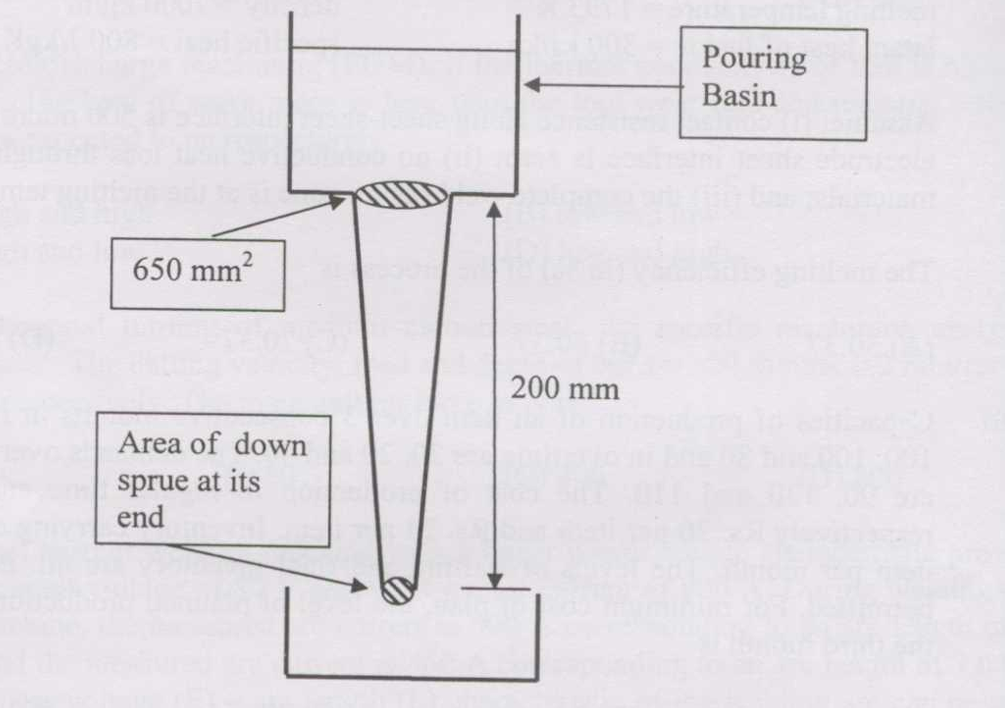
\includegraphics[width=0.8\textwidth]{Fig 9.png}
    \caption{}
    \label{fig:question42}
\end{figure}

\begin{multicols}{4}
\begin{enumerate}
\item $ \frac{1}{2\pi} \sqrt{\frac{k}{m}} $  
\item $ \frac{1}{2\pi} \sqrt{\frac{2k}{m}} $  
\item $ \frac{1}{2\pi} \sqrt{\frac{2k}{3m}} $  
\item $ \frac{1}{2\pi} \sqrt{\frac{3k}{2m}} $  
\end{enumerate}
\end{multicols}   
\hfill (GATE ME 2011)

\item A 1 kg block resting on a surface with coefficient of friction $ \mu = 0.1 $. A force of 0.8 N is applied to the block as shown in the figure. The friction force is:

\begin{figure}[H]
    \centering
    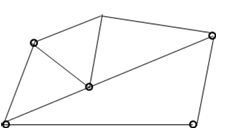
\includegraphics[width=0.8\textwidth]{Fig 10.png}
    \caption{}
    \label{fig:question43}
\end{figure}

\begin{multicols}{4}
\begin{enumerate}
\item 0  
\item 0.8 N  
\item 0.98 N  
\item 1.2 N  
\end{enumerate}
\end{multicols}   
\hfill (GATE ME 2011)

\item Consider the system of equations:  

$ 2x_1 + x_2 + x_3 = 0 $,  

$ x_2 - x_3 = 0 $,  

$ x_1 + x_2 = 0 $.  

This system has
\begin{multicols}{2}
\begin{enumerate}
\item a unique solution  
\item no solution  
\item infinite number of solutions  
\item five solutions  
\end{enumerate}
\end{multicols}   
\hfill (GATE ME 2011)

\item A single-point cutting tool with 12° rake angle is used to machine a steel work-piece. The depth of cut is 0.81 mm. The chip thickness under orthogonal machining condition is 1.8 mm. The shear angle is approximately
\begin{multicols}{4}
\begin{enumerate}
\item 22°
\item 26°
\item 56°
\item 76°
\end{enumerate}
\end{multicols}   
\hfill (GATE ME 2011)

\item Match the following non-traditional machining processes with the corresponding material removal mechanisms:

\begin{tabular}{|c|c|}
\hline
Machining process              & Mechanism of material removal \\
\hline
P. Chemical machining          & 1. Erosion \\
\hline
Q. Electro-chemical machining  & 2. Corrosive reaction \\
\hline
R. Electro-discharge machining & 3. Ion displacement \\
\hline
S. Ultrasonic machining        & 4. Fusion and vaporiazation \\
\hline
\end{tabular}

\begin{multicols}{2}
\begin{enumerate}
\item P-2, Q-3, R-4, S-1
\item P-3, Q-2, R-4, S-1
\item P-2, Q-4, R-3, S-1
\item P-2, Q-3, R-1, S-4
\end{enumerate}
\end{multicols}   
\hfill (GATE ME 2011)

\item A cubic casting of 50 mm side undergoes volumetric solidification shrinkage and contraction of $4\% and 6\% $ respectively. No riser is used. Assume uniform cooling in all directions. The side of the cube after solidification and contraction is
\begin{multicols}{4}
\begin{enumerate}
\item 48.32 mm
\item 49.90 mm
\item 49.94 mm
\item 49.96 mm
\end{enumerate}
\end{multicols}   
\hfill (GATE ME 2011)

\textbf{Common Data Questions}

\textbf{Common Data for Questions 48 and 49:} 

In an experimental set-up, air flows between two stations P and Q adiabatically. The direction of flow depends on the pressure and temperature conditions maintained at P and Q.  
The conditions at station P are:  
$P_P = 150\,\text{kPa} $ and $350\,\text{K}$  
The temperature at station Q is:  
$T_Q = 300\,\text{K}$.

The following are the properties and relations pertaining to air:

Specific heat at constant pressure, $c_p = 1.005\,\text{kJ/kg·K},$

Specific heat at constant volume,$ c_v = 0.718\,\text{kJ/kg·K},$ 

Characteristic gas constant, $R = 0.287\,\text{kJ/kg·K}$

Enthalpy, $h = c_p T, $

Internal energy, $u = c_v T$.


\item If the air has to flow from station P to station Q, the maximum possible value of pressure in kPa at station Q is close to:

\begin{multicols}{2}
\begin{enumerate}
\item 50  
\item 87  
\item 128  
\item 150  
\end{enumerate}
\end{multicols}    
\hfill (GATE ME 2011)

\item If the pressure at station Q is 50 kPa, the change in entropy  ($ s_Q - s_P $) in kJ/kgK is:

\begin{multicols}{4}
\begin{enumerate}
\item $-0.155$  
\item 0  
\item 0.160  
\item 0.355  
\end{enumerate}
\end{multicols}    
\hfill (GATE ME 2011)

\textbf{Common Data for Questions 50 and 51:} 

 One unit of product P1 requires 3 kg of resource R1 and 1 kg of resource R2. One unit of product P2 requires 2 kg of resource R1 and 2 kg of resource R2. The profits per unit by selling product P1 and P2 are Rs. 2000 and Rs. 3000 respectively. The manufacturer has 90 kg of resource R1 and 100 kg of resource R2.
\item The unit worth of resource R2, i.e. dual price of resource R2 in Rs. per kg is
\begin{multicols}{4}
\begin{enumerate}
\item 0
\item 1350
\item 1500
\item 2000
\end{enumerate}
\end{multicols}    
\hfill (GATE ME 2011)

\item The manufacturer can make a maximum profit of Rs.
\begin{multicols}{4}
\begin{enumerate}
\item 60000
\item 135000
\item 150000
\item 200000
\end{enumerate}
\end{multicols}    
\hfill (GATE ME 2011)

\textbf{Linked Answer Questions}

\textbf{Statement for Linked Answer Questions 52 and 53:}

 A triangular-shaped cantilever beam of uniform-thickness is shown in the figure. The Young's modulus of the material of the beam is $ E $. A concentrated load $ P $ is applied at the free end of the beam.

 \begin{figure}[H]
    \centering
    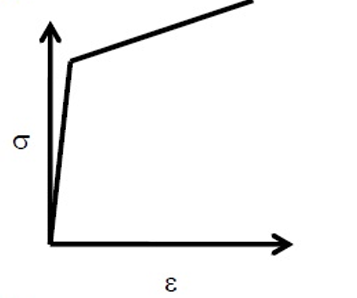
\includegraphics[width=0.8\textwidth]{Fig 11.png}
    \caption{}
    \label{fig:question52,53}
\end{figure}

\item The area moment of inertia about the neutral axis of a cross-section at a distance $ x $ measured from the free end is
\begin{multicols}{4}
\begin{enumerate}
\item $ \frac{bxt^3}{6l} $
\item $ \frac{bxt^3}{12l} $
\item $ \frac{bxt^3}{24l} $
\item $ \frac{xt^3}{12} $
\end{enumerate}
\end{multicols}   
\hfill (GATE ME 2011)

\item The maximum deflection of the beam is
\begin{multicols}{4}
\begin{enumerate}
\item $ \frac{24Pl^3}{Ebt^3} $
\item $ \frac{12Pl^3}{Ebt^3} $
\item $ \frac{8Pl^3}{Ebt^3} $
\item $ \frac{6Pl^3}{Ebt^3} $
\end{enumerate}
\end{multicols}   
\hfill (GATE ME 2011)

\textbf{Statement for Linked Answer Questions 54 and 55:}

The temperature and pressure of air in a large reservoir are 400 K and 3 bar respectively. A converging-diverging nozzle of exit area 0.005 m² is fitted to the wall of the reservoir as shown in the figure. The static pressure of air at the exit section for isentropic flow through the nozzle is 50 kPa. The characteristic gas constant and the ratio of specific heats of air are 0.287 kJ/kgK and 1.4 respectively.

\begin{figure}[H]
    \centering
    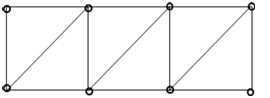
\includegraphics[width=0.8\textwidth]{Fig 12.png}
    \caption{}
    \label{fig:question54,55}
\end{figure}

\item The density of air in kg/m³ at the nozzle exit is
\begin{multicols}{4}
\begin{enumerate}
\item 0.560
\item 0.600
\item 0.727
\item 0.800
\end{enumerate}
\end{multicols}   
\hfill (GATE ME 2011)

\item The mass flow rate of air through the nozzle in kg/s is  \begin{multicols}{4}
\begin{enumerate}
\item 1.30
\item 1.77
\item 1.85
\item 2.06
\end{enumerate}
\end{multicols}   
\hfill (GATE ME 2011)

\textbf{General Aptitude (GA) Questions}

\textbf{Q. 56 - Q. 60 carry one mark each.}

  \item Choose the word from the options given below that is most nearly opposite in meaning to the given word:
  
\textbf{Amalgamate}
    \begin{enumerate}
      \item merge
      \item split
      \item collect
      \item separate
    \end{enumerate}
    \hfill (GATE ME 2011)

  \item Which of the following options is the closest in the meaning to the word below: 
\textbf{Inexplicable}
    \begin{enumerate}
      \item Incomprehensible
      \item Indelible
      \item Inextricable
      \item Infallible
    \end{enumerate}
    \hfill (GATE ME 2011)

  \item If $\log(P) = \frac{1}{2} \log(Q) = \frac{1}{3} \log(R)$, then which of the following options is \textbf{TRUE}?
  \begin{multicols}{4}
    \begin{enumerate}
      \item $P^2 = Q^3 R^2$
      \item $Q^2 = PR$
      \item $Q^2 = R^3 P$
      \item $R = P^2 Q^2$
    \end{enumerate}
  \end{multicols}   
  \hfill (GATE ME 2011)

  \item Choose the most appropriate word(s) from the options given below to complete the following sentence.
  
 \textbf{I contemplated ---------- Singapore for my vacation but decided against it.}
 
    \begin{enumerate}
      \item to visit
      \item having to visit
      \item visiting
      \item for a visit
    \end{enumerate}
    \hfill (GATE ME 2011)
    
  \item Choose the most appropriate word from the options given below to complete the following sentence.
  
 \textbf{If you are trying to make a strong impression on your audience, you cannot do so by being understated, tentative or ----------.}

    \begin{enumerate}
      \item hyperbolic
      \item restrained
      \item argumentative
      \item indifferent
    \end{enumerate}
    \hfill (GATE ME 2011)

\textbf{Q. 61 - Q. 65 carry two marks each.}

\item A container originally contains 10 litres of pure spirit. From this container 1 litre of spirit is replaced with 1 litre of water. Subsequently, 1 litre of the mixture is again replaced with 1 litre of water and this process is repeated one more time. How much spirit is now left in the container?
\begin{multicols}{4}
  \begin{enumerate}
    \item 7.58 litres  
    \item 7.84 litres  
    \item 7 litres  
    \item 7.29 litres  
  \end{enumerate}
\end{multicols}     
\hfill (GATE ME 2011)

\item \textbf{Few school curricula include a unit on how to deal with bereavement and grief, and yet all students at some point in their lives suffer from losses through death and parting.}

Based on the above passage, which topic would not be included in a unit on bereavement?
  \begin{enumerate}
    \item how to write a letter of condolence  
    \item what emotional stages are passed through in the healing process  
    \item what the leading causes of death are  
    \item how to give support to a grieving friend  
  \end{enumerate}
  \hfill (GATE ME 2011)

\item P, Q, R and S are four types of dangerous microbes recently found in a human habitat. The area of each circle with its diameter printed in brackets represents the growth of a single microbe surviving human immunity system within 24 hours of entering the body. The danger to human beings varies proportionately with the toxicity, potency and growth attributed to a microbe shown in the figure below:

\begin{figure}[H]
    \centering
    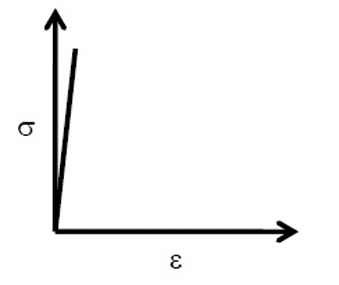
\includegraphics[width=0.8\textwidth]{Fig 13.png}
    \caption{}
    \label{fig:question63}
\end{figure}

A pharmaceutical company is contemplating the development of a vaccine against the most dangerous microbe. Which microbe should the company target in its first attempt?
\begin{multicols}{4}
  \begin{enumerate}
    \item P  
    \item Q  
    \item R  
    \item S  
  \end{enumerate}
\end{multicols}    
\hfill (GATE ME 2011)

\item The variable cost (V) of manufacturing a product varies according to the equation $ V = 4q $, where $ q $ is the quantity produced. The fixed cost (F) of production of the same product reduces with $ q $ according to the equation $ F = \frac{100}{q} $. How many units should be produced to minimize the total cost ($ V + F $)?
\begin{multicols}{4}
  \begin{enumerate}
    \item 5  
    \item 4  
    \item 7  
    \item 6  
  \end{enumerate}
\end{multicols}    
\hfill (GATE ME 2011)

\item A transporter receives the same number of orders each day. Currently, he has some pending orders (backlog) to be shipped. If he uses 7 trucks, then at the end of the 4th day he can clear all the orders. Alternatively, if he uses only 3 trucks, then all the orders are cleared at the end of the 10th day. What is the minimum number of trucks required so that there will be no pending order at the end of the 5th day?
\begin{multicols}{4}
  \begin{enumerate}
    \item 4  
    \item 5  
    \item 6  
    \item 7  
  \end{enumerate}
\end{multicols}     
\hfill (GATE ME 2011)

\end{enumerate}
\end{document}